\documentclass[12pt]{article}
\usepackage{sbc-template}
\usepackage[T1]{fontenc}
\usepackage[utf8]{inputenc}
\usepackage[brazil]{babel}
\usepackage{graphicx,url}
\usepackage[hidelinks]{hyperref}
\newcommand{\doilink}[1]{\href{https://doi.org/#1}{\nolinkurl{#1}}}
\sloppy

\title{MindScreen: um protótipo de reflexão familiar sobre rotina digital informado por uma análise da NSCH (2020--2024)}
\author{Kauan Edson Leonel Lira\inst{1}, Eduarda Gonçalves Luiz de Andrade\inst{1}}
\address{Instituto Federal de São Paulo -- Câmpus Caraguatatuba -- Brasil}

\begin{document}
\maketitle
\begin{abstract}
We present MindScreen, a family reflection prototype informed by the US National Survey of Children's Health (2020--2024, 166,343 records aged 6--17). In survey-weighted models, adjusted odds ratios for four or more hours of screen time versus less than one were 1.19 (95\% CI 0.83--1.69) for current depression and 1.44 (1.22--1.70) for current anxiety, as reported by caregivers. Adding screen time changed exploratory 2024 ROC AUC by less than 0.005 for either outcome. The prototype offers a voluntary diary and family planning. Family use remains unevaluated.
\end{abstract}
\begin{resumo}
Apresentamos o MindScreen, protótipo de reflexão familiar informado pela National Survey of Children's Health dos EUA (2020--2024, 166.343 registros de 6 a 17 anos). Com ponderação e ajuste, quatro horas ou mais de tela frente a menos de uma apresentaram razões de chances de 1,19 (IC95\% 0,83--1,69) para relato de depressão atual e 1,44 (1,22--1,70) para ansiedade atual. Incluir tempo de tela alterou a ROC AUC exploratória de 2024 em menos de 0,005 para ambos. O protótipo oferece diário voluntário e plano familiar. Seu uso com famílias permanece por avaliar.
\end{resumo}

\section{Introdução}
Uma estimativa diária de tempo de tela resume atividades tão distintas quanto jogar, assistir a vídeos ou conversar com amigos. Essa medida ajuda a descrever a rotina, mas oferece pouca informação sobre a experiência digital em si, como conteúdo, finalidade e contexto. Entre crianças de 9 a 10 anos, \cite{paulich2021} encontraram associações de magnitude modesta entre tempo de tela e indicadores acadêmicos, sociais e de saúde mental. Na prática, uma ferramenta que acompanha hábitos precisa preservar a diferença entre observar durações e interpretar o que elas significam para uma família.

A \textit{National Survey of Children's Health} (NSCH) reúne informações de responsáveis sobre a saúde e o contexto de crianças que residem em domicílios nos Estados Unidos \cite{censusdata,censusguide}. Suas edições públicas permitem examinar a distribuição dos relatos e testar o quanto uma medida de duração informa modelos com outras características da rotina. Perguntamos como as categorias de tela se associam aos relatos atuais de depressão e ansiedade após ajuste e consideração do desenho amostral. Também estimamos quanto essa variável acrescenta à classificação dos relatos na avaliação exploratória de 2024. Os modelos classificam condições contemporâneas à exposição. A utilidade de uma interface familiar exige evidência de outra natureza.

Essa distinção orienta o MindScreen. Para responsáveis, crianças e adolescentes conversarem sobre a rotina, o protótipo organiza registros voluntários, visualizações e combinados escolhidos em família. As contribuições são a harmonização de cinco edições, a comparação entre resultados amostrais e ponderados, a avaliação da contribuição incremental de tempo de tela e a implementação de um fluxo verificável. As seções seguintes descrevem a literatura, os métodos, os resultados e as implicações para o protótipo.

\section{Trabalhos relacionados}
\subsection{Tempo de tela e indicadores de saúde mental}
A literatura oferece resultados diferentes conforme o que se mede e quando se mede. \cite{boers2019} acompanharam adolescentes canadenses e distinguiram atividades digitais e associações entre indivíduos e dentro do mesmo indivíduo. Uma metanálise de coortes prospectivas identificou associação entre maior exposição inicial e depressão posterior, com elevada heterogeneidade \cite{gao2024}. Já a revisão longitudinal de \cite{tang2021} encontrou associações pequenas ou muito pequenas para sintomas depressivos posteriores e evidência limitada para ansiedade. Na coorte australiana de \cite{li2025}, as associações foram mais fracas no seguimento que no corte transversal, sem associação longitudinal para ansiedade em 12 meses. Sintomas em escalas, funcionamento psicossocial e condições relatadas por responsáveis são desfechos distintos.

Essa diversidade também aparece nos estudos sobre redes sociais, que investigam apenas parte do uso de telas. \cite{kreski2021} encontraram associações pouco consistentes entre uso diário de redes e sintomas depressivos em adolescentes norte-americanos. \cite{valkenburg2022} identificaram interpretações divergentes entre revisões, muitas delas descrevendo associações fracas. A qualidade da evidência e a variação individual merecem atenção ao interpretar médias \cite{stiglic2019,orben2020}. Em uma edição anterior da NSCH, \cite{przybylski2020} estudaram tempo de tela e funcionamento psicossocial, com medidas diferentes das adotadas aqui. A literatura sobre sono também documenta associações com uso de tela e limitações de mensuração \cite{hale2015}, o que motiva considerar as duas dimensões da rotina sem assumir uma direção causal.

A própria duração é sensível ao instrumento. \cite{parry2021} encontraram discrepâncias entre autorrelatos e registros digitais em uma metanálise. Isso oferece uma razão para tratar horas relatadas como aproximações, embora o estudo não quantifique o erro de relato dos responsáveis na NSCH. Uma categoria aberta como quatro horas ou mais também reúne durações e experiências distintas. Assim, qualquer interpretação dos coeficientes depende do que foi perguntado e do contexto em que o tempo foi relatado.

Na coorte ABCD, \cite{nagata2024} encontraram associações prospectivas pequenas entre exposição a telas e sintomas em dois anos. Entre as atividades mais associadas a sintomas depressivos estavam chamadas de vídeo, mensagens, vídeos e jogos. Em outro contexto, \cite{george2020} encontraram pouca evidência de associação média entre acesso e uso digitais e bem-estar entre adolescentes da Carolina do Norte, mas observaram mais experiências negativas relatadas por jovens de famílias em desvantagem econômica. Esses estudos mostram por que duração, tipo de uso e oportunidades familiares merecem tratamento distinto. A NSCH utilizada aqui não permite atribuir a diferença entre categorias de duração a uma atividade específica.

\subsection{Autorregistro e planejamento familiar}
A pesquisa em informática pessoal situa o autorregistro em um processo que envolve coleta, organização, reflexão e ação \cite{li2010informatica}. Pausas e retomadas de uso fazem parte desse processo \cite{epstein2015}. Essas ideias ajudam a interpretar o fluxo do MindScreen, no qual registros parciais podem servir de ponto de partida para uma conversa. A Academia Americana de Pediatria orienta que famílias construam um plano de mídia adequado às suas prioridades e reservem espaço para outras atividades \cite{aap2026}. Em um ensaio randomizado com responsáveis e adolescentes de 12 a 17 anos, completar um plano familiar de mídia não produziu diferença estatisticamente detectável no envolvimento com as regras de mídia \cite{moreno2021}. A presença de um plano na interface, portanto, é uma funcionalidade a avaliar, com resultados de uso próprios.

\section{Materiais e métodos}
\subsection{Fonte, seleção e harmonização}
Os arquivos públicos \textit{topical} da NSCH de 2020 a 2024 foram analisados como cortes transversais anuais. A janela corresponde às cinco edições harmonizadas no projeto. As quatro primeiras serviram ao desenvolvimento dos classificadores e a última à comparação temporal. A NSCH cobre crianças não institucionalizadas que residem em domicílios nos Estados Unidos. Um responsável informa sobre a criança selecionada. O recorte de 6 a 17 anos corresponde aos formulários T2 e T3 e mantém o universo comum dos itens de rotina \cite{census2020,census2021,census2022,census2023,census2024,censusaccuracy2024}.

A harmonização verificou identificadores, idade, formulário, estrato, peso e valores permitidos. Para cada edição, foram confrontados contagens e totais ponderados por sexo e frequências de \texttt{SCREENTIME} com os controles publicados pelo Census. O guia exige as versões aprimoradas de 2020 e 2021 na combinação com anos posteriores. Os CSVs locais têm a nomenclatura esperada e controles compatíveis com os pesos publicados. A procedência integral dos arquivos originais ainda carece de confirmação independente \cite{censusguide}.

O item \texttt{SCREENTIME} pergunta pelo uso de televisão, computador, celular ou outros dispositivos para atividades como assistir a programas, jogar, acessar a internet ou usar redes sociais na maioria dos dias de semana. As cinco categorias são menos de uma hora, uma, duas, três e quatro horas ou mais. A categoria superior permaneceu aberta. A instrução de excluir tarefas escolares aparece explicitamente em 2024. Por isso, tratamos o item como aproximação do uso recreativo e repetimos a análise ajustada sem 2024 \cite{census2020,census2021,census2022,census2023,census2024}.

Os pares \texttt{K2Q32A/B} e \texttt{K2Q33A/B} distinguem histórico informado por profissional e condição atual de depressão e ansiedade. Respostas afirmativas compatíveis nos dois itens definiram o relato positivo. Uma resposta histórica negativa com salto documentado, ou uma resposta atual negativa compatível, definiu ausência atual. Histórico desconhecido, condição atual indeterminada e combinações inconsistentes permaneceram ausentes. Campos vazios nos CSVs nem sempre preservam o motivo da ausência. Os desfechos refletem informação de responsáveis, sujeita ao reconhecimento da condição, acesso a atendimento e recordação. A pesquisa não realiza avaliação clínica individual.

\subsection{Associação amostral e análise de desenho}
A análise original ajustou regressões logísticas separadas, sem penalização, por casos completos de 2020--2023. Os modelos incluíram idade em anos e indicadores para sexo, sono, atividade física, dificuldade para fazer amigos, ano e categoria de tela. A referência foi menos de uma hora. As razões de chances (OR) correspondem aos exponenciais dos coeficientes das categorias e descrevem contrastes condicionados às covariáveis. A regressão original usou pesos uniformes e é apresentada como descrição da amostra, sem intervalos de confiança de desenho.

Os itens de rotina são \texttt{HOURSLEEP} (duração na maioria das noites úteis da última semana), \texttt{PHYSACTIV} (dias da última semana com pelo menos 60 minutos de atividade) e \texttt{MAKEFRIEND} (dificuldade para fazer ou manter amigos, em comparação com crianças da mesma idade). \texttt{SC\_AGE\_YEARS} e \texttt{SC\_SEX} descrevem a idade e o sexo registrados \cite{census2024}.

Na análise complementar, as colunas de desenho dos CSVs foram confrontadas com os registros harmonizados de 6 a 17 anos. Foram usados o peso final infantil \texttt{FWC} dividido pelo número de edições, estratos formados pelo cruzamento de \texttt{FIPSST} e \texttt{STRATUM}, e domicílio (\texttt{HHID}) como unidade primária. A implementação segue o exemplo multianual do Census para estratificação e linearização de Taylor sob aproximação com reposição \cite{censusguide,censusaccuracy2024,lumley2004}. Foi verificada a unicidade do identificador domiciliar entre edições. O cálculo de variância preservou todas as unidades do arquivo combinado, com contribuição zero fora de cada domínio. Cada prevalência usa a soma de pesos dos relatos positivos dividida pela soma de pesos no domínio com tela e desfecho conhecidos. Também foram calculados contrastes descritivos por faixa etária para as duas categorias extremas.

As regressões ponderadas foram ajustadas por pseudoverossimilhança, com variância sanduíche obtida da linearização dos escores centrados por estrato. Os IC95\% foram calculados na escala logito para proporções e na escala log-OR para os coeficientes, com quantil $t$ e graus de liberdade do desenho (unidades menos estratos). Na mesma amostra de casos completos por desfecho, comparamos um modelo bruto, um com idade, sexo e ano, e um com ajuste adicional por duração do sono, dias de atividade física e dificuldade para fazer amigos. Idade foi contínua e centrada em 12 anos. As demais variáveis entraram como indicadores, com a primeira categoria observada em ordem de código como referência. O ajuste demográfico considera diferenças de composição e edição. O ajuste de rotina caracteriza um contraste condicionado a medidas contemporâneas, que podem ocupar posições distintas na relação entre exposição e desfecho. Foi calculado o maior fator de inflação da variância (VIF) dos indicadores na matriz ponderada. Os intervalos são pontuais e exploratórios, sem correção por comparações múltiplas. Não se ajustou por condição socioeconômica nem se imputaram itens nesta análise.

\subsection{Modelagem e avaliação temporal}

A comparação empregou dois conjuntos de variáveis: A, com tempo de tela, e B, sem tempo de tela. Ambos incluíram idade, sexo, sono, atividade física e dificuldade para fazer amigos. Os itens usados para construir os desfechos, os identificadores e os pesos foram excluídos dos preditores. Ainda pode haver proximidade informacional com o desfecho, por exemplo entre dificuldade para fazer amigos e uma condição atual, pois todos os atributos são contemporâneos. Regressão logística, floresta aleatória e XGBoost foram comparados com um classificador que usa a frequência da classe positiva no desenvolvimento como escore constante.

A seleção por área sob a curva ROC (ROC AUC) usou cinco partições estratificadas de 2020--2023, idênticas entre A e B para cada desfecho, com semente 42. Nas partições, a idade foi imputada pela mediana, os faltantes categóricos receberam indicador próprio e a codificação foi binária por categoria. Apenas a regressão logística recebeu padronização numérica. A busca variou $C$ da logística (0,1 e 1), profundidade da floresta (sem limite ou 10), profundidade do XGBoost (3 ou 5) e sua taxa de aprendizado (0,05 ou 0,10). Floresta e XGBoost usaram 200 árvores, com mínimo de dez casos por folha na floresta. A busca comparou pesos de classe uniformes e balanceados na logística e na floresta, e fator da classe positiva de 1 ou a razão entre negativos e positivos no desenvolvimento no XGBoost. Esses pesos de classe não correspondem aos pesos do desenho da NSCH. O limiar de cada modelo maximizou F1 nas previsões fora da partição, nas mesmas divisões usadas para selecionar hiperparâmetros. Essa reutilização limita a independência da estimativa de desenvolvimento.

A avaliação utilizou, por desfecho, os registros de 2024 com condição determinada, mantendo os preditores ausentes tratáveis pelo modelo. A ROC AUC mede ordenação dos escores. A precisão média (AP) resume a curva precisão--sensibilidade e deve ser interpretada considerando a frequência de positivos \cite{saito2015}. Precisão, sensibilidade e F1 são medidas no limiar escolhido. Para o contraste A menos B foram usados intervalos percentílicos por bootstrap pareado de registros de 2024, em 1.000 reamostras, com semente 42. Esses intervalos condicionam-se aos modelos ajustados e ignoram o desenho da pesquisa. O protocolo de limiar e de ponderação de classes do XGBoost foi revisto após a análise inicial de 2024. Assim, a avaliação dessa edição é temporal e exploratória, com exposição anterior aos seus resultados.

A Tabela~\ref{tab:predicao} usa a versão 2 dos modelos (\texttt{v2\_limiar\_cv}). A versão 1, com limiar 0,5, motivou a revisão do protocolo após baixo reconhecimento da classe positiva. Na versão 2, as escolhas numéricas de hiperparâmetros e limiar usaram a janela de desenvolvimento. Isso não restaura a independência de 2024. O repositório também registra uma versão 3 com calibração pós-hoc. Essa etapa comparou ausência de calibração, sigmoide e regressão isotônica por escore de Brier, usando previsões de 2020--2023 e ajuste cruzado dos calibradores. O escore de Brier corresponde ao erro quadrático médio entre o escore e o rótulo binário. São reportadas separadamente as mudanças de calibração em 2024. Nenhum desses procedimentos avaliou implantação clínica ou transportabilidade.

\subsection{Implementação e verificação do protótipo}
O protótipo usa Python e Streamlit. A Figura~\ref{fig:fluxo-produto} apresenta as responsabilidades de cada componente. Na navegação, o início explica a proposta, o diário coleta entradas, o histórico as apresenta, o plano organiza combinados e a página de pesquisa descreve a origem da evidência. As regras do diário ficam em \texttt{mindscreen.rotina}, separadas dos componentes de apresentação. O diário aceita duração estimada de tela recreativa no dia, horas de sono da noite anterior e atividades escolhidas de uma lista. Aceita ao menos um campo preenchido, datas até o dia corrente e durações de zero a 24 horas. Registrar a mesma data substitui a entrada anterior. O histórico preserva a diferença entre ausência e zero, com gráficos de pontos Plotly para as durações e tabela com atividades. As entradas têm períodos de referência diferentes dos itens da NSCH.

O plano oferece combinados editáveis de uma lista e perguntas para conversar sobre atividades e prioridades. Os requisitos de privacidade do protótipo são minimizar os campos e manter registros e escolhas em memória na sessão Streamlit. A barra lateral permite removê-los. O encerramento da sessão pode apagar o histórico e a interface carece de acompanhamento persistente entre sessões. A aplicação familiar dispensa arquivos da NSCH e classificadores para funcionar. A verificação funcional utilizou \texttt{pytest} nas regras e \texttt{AppTest} do Streamlit para percorrer diário, histórico, plano e exclusão. Os critérios foram aceitar entradas válidas, preservar itens ausentes, recusar entradas inválidas, exibir o valor salvo, manter a seleção do plano ao navegar e remover o histórico ao apagar. A revisão não envolveu participantes.

\begin{figure}[htbp]
\centering
\small
\begin{tabular}{ccc}
\fbox{\parbox[c][3.6em][c]{0.37\linewidth}{\centering\textbf{Interface Streamlit}\\Início, diário, histórico,\\plano e página de pesquisa}} & $\leftrightarrow$ &
\fbox{\parbox[c][3.6em][c]{0.40\linewidth}{\centering\textbf{Regras de domínio}\\Validação, atualização\\por data e organização}} \\
$\updownarrow$ & & \\
\fbox{\parbox[c][3.6em][c]{0.37\linewidth}{\centering\textbf{Sessão em memória}\\Entradas e combinados,\\com exclusão pela barra lateral}} & $\longrightarrow$ &
\fbox{\parbox[c][3.6em][c]{0.40\linewidth}{\centering\textbf{Histórico}\\Tabela de atividades e\\gráficos para tela e sono}}
\end{tabular}
\caption{Componentes do fluxo familiar. A interface envia entradas às regras, guarda o resultado na sessão e usa os registros validados para montar o histórico.}
\label{fig:fluxo-produto}
\end{figure}

\section{Resultados}
\subsection{Composição da amostra e associações}
Das cinco edições, 166.343 registros atenderam ao recorte etário (Tabela~\ref{tab:fluxo}). Havia 2.705 registros sem categoria de tela. Para depressão atual, 11.193 tinham relato positivo, 154.185 negativo e 965 indeterminado. Para ansiedade atual, foram 26.051 positivos, 138.650 negativos e 1.642 indeterminados. Ausências podem se sobrepor.

\begin{table}[htbp]
\centering
\caption{Registros por edição antes e após a seleção etária.}
\label{tab:fluxo}
\begin{tabular}{lrrrrr}\hline
Ano & Origem & 6--17 anos & 12--17 anos & Sexo feminino & Tela ausente \\\hline
2020 & 42.777 & 30.636 & 17.539 & 14.783 & 560 \\
2021 & 50.892 & 30.173 & 16.166 & 14.434 & 531 \\
2022 & 54.103 & 34.362 & 19.028 & 16.532 & 548 \\
2023 & 55.162 & 33.638 & 18.397 & 16.198 & 491 \\
2024 & 51.375 & 37.534 & 21.960 & 18.215 & 575 \\\hline
Total & 254.309 & 166.343 & 93.090 & 80.162 & 2.705 \\\hline
\end{tabular}

\smallskip{\footnotesize Contagens não ponderadas. A partir da terceira coluna, o universo é o recorte de 6 a 17 anos. Fonte: arquivos \textit{topical} e Parquet harmonizado.}
\end{table}

Entre registros com tempo informado, quatro horas ou mais representaram 34,8\% em 2020, 26,5\% em 2023 e 31,1\% em 2024. Essas diferenças descrevem a composição das amostras anuais. A alteração do enunciado em 2024 limita sua interpretação como tendência. Em 2020--2023, havia 128.809 registros no recorte. Restaram 124.795 casos completos para depressão e 124.299 para ansiedade. As maiores OR sem ponderação foram observadas para quatro horas ou mais frente a menos de uma hora, com 1,79 para depressão e 1,65 para ansiedade.

\subsection{Resultados com ponderação e variância de desenho}
O desenho combinado incluiu 254.309 unidades domiciliares em 102 estratos. A Tabela~\ref{tab:prev} mostra as prevalências ponderadas entre crianças com tela e desfecho conhecidos. A prevalência de relato de depressão foi de 3,2\% na referência e 9,3\% na categoria mais alta, enquanto a de ansiedade foi de 8,1\% e 17,8\%. A categoria de uma hora apresentou estimativas inferiores às da referência, o que desaconselha resumir o padrão como um gradiente monotônico. Nas categorias extremas, as estimativas estratificadas de depressão passaram de 1,2\% para 3,7\% entre 6 e 11 anos, e de 7,4\% para 11,9\% entre 12 e 17. Para ansiedade, os pares foram 6,9\% e 12,3\%, e 10,8\% e 20,5\%, respectivamente. São comparações descritivas sem teste de interação por idade.

\begin{table}[htbp]
\centering
\caption{Prevalência ponderada de relatos atuais segundo categoria de tela, NSCH 2020--2024.}
\label{tab:prev}
\begin{tabular}{lrrrr}\hline
Tela & $n$ (depr.) & Depr., \% (IC95\%) & $n$ (ans.) & Ans., \% (IC95\%) \\\hline
Menos de 1 h & 9.729 & 3,2 (2,4--4,3) & 9.713 & 8,1 (7,1--9,3) \\
1 h & 20.690 & 2,0 (1,7--2,4) & 20.634 & 7,8 (7,2--8,5) \\
2 h & 46.438 & 3,3 (3,0--3,7) & 46.265 & 9,5 (9,1--10,0) \\
3 h & 37.082 & 4,6 (4,2--5,0) & 36.903 & 11,7 (11,2--12,3) \\
4 h ou mais & 48.769 & 9,3 (8,8--9,8) & 48.537 & 17,8 (17,2--18,5) \\\hline
\end{tabular}

\smallskip{\footnotesize $n$ não ponderado por desfecho, com categoria de tela e desfecho conhecidos. IC95\% por linearização de Taylor. Fonte: análise de desenho dos arquivos \textit{topical}.}
\end{table}

O ajuste mudou a magnitude dos contrastes (Tabela~\ref{tab:ajustes}). Em 2020--2024, os casos completos foram 161.150 para depressão e 160.512 para ansiedade. O ajuste completo elevou o VIF máximo de cerca de 4,1 no modelo demográfico para 17,62 e 17,74, respectivamente, no indicador de oito horas de sono. Os VIFs dependem da codificação dos indicadores. O resultado reforça a utilidade de apresentar os dois conjuntos de ajuste e interpretar com cautela os coeficientes das categorias de rotina. Para o contraste extremo, o IC95\% de depressão após ajuste completo incluiu 1, enquanto o de ansiedade permaneceu acima de 1. Na mesma janela de 2020--2023 e com os mesmos denominadores da análise original, a ponderação também reduziu os pontos estimados para ambos os desfechos.

A Figura~\ref{fig:or} detalha o ajuste completo nas categorias intermediárias. Os intervalos de ansiedade nas categorias de três horas e de quatro horas ou mais ficaram acima de 1. Para depressão, a única categoria cujo intervalo não incluiu 1 foi uma hora, com OR abaixo de 1. Esse contraste deve ser interpretado com cautela diante das comparações múltiplas e da ausência de ajuste socioeconômico.

\begin{figure}[htbp]
\centering
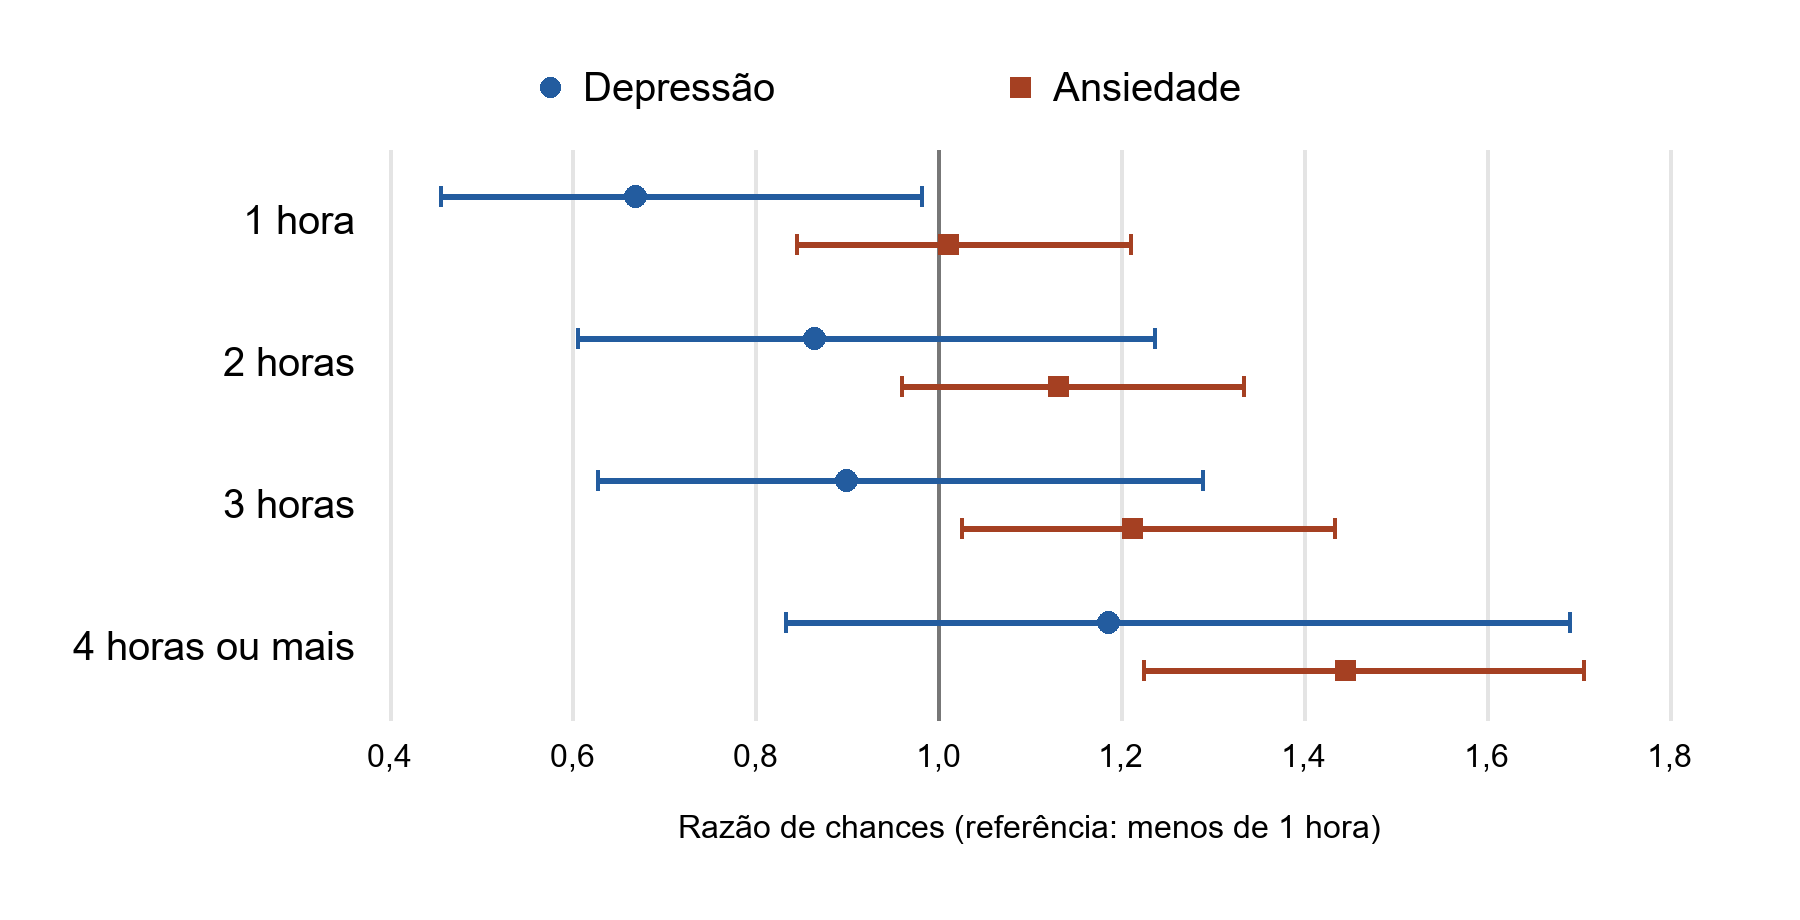
\includegraphics[width=0.92\linewidth]{figuras/associacao_ponderada.png}
\caption{Razões de chances ponderadas e IC95\% para relatos atuais de depressão e ansiedade, 2020--2024. Ajuste por idade, sexo, sono, atividade física, dificuldade de fazer ou manter amigos e ano. Fonte: análise de desenho dos arquivos \textit{topical}.}
\label{fig:or}
\end{figure}

\begin{table}[htbp]
\centering
\caption{Razões de chances ponderadas para quatro horas ou mais de tela frente a menos de uma hora.}
\label{tab:ajustes}
\begin{tabular}{llrr}\hline
Edições & Ajuste & Depressão (IC95\%) & Ansiedade (IC95\%) \\\hline
2020--2024 & Bruto & 3,07 (2,25--4,19) & 2,41 (2,08--2,80) \\
2020--2024 & Idade, sexo, ano & 1,84 (1,34--2,53) & 1,95 (1,67--2,27) \\
2020--2024 & Completo & 1,19 (0,83--1,69) & 1,44 (1,22--1,70) \\
2020--2023 & Completo & 1,27 (0,84--1,91) & 1,45 (1,20--1,75) \\\hline
\end{tabular}

\smallskip{\footnotesize Ajuste completo acrescenta sono, atividade física e dificuldade para fazer amigos. Modelos de 2020--2024 compartilham o mesmo conjunto de casos completos por desfecho. Fonte: análise de desenho dos arquivos \textit{topical}.}
\end{table}

\subsection{Contribuição incremental de tempo de tela}
O XGBoost foi selecionado no desenvolvimento para ambos os desfechos e conjuntos de preditores. Na avaliação de 2024, havia 2.537 relatos positivos entre 37.275 registros de depressão determinada e 6.450 entre 37.128 registros de ansiedade determinada. A Tabela~\ref{tab:predicao} apresenta as métricas dos modelos selecionados.

\begin{table}[htbp]
\centering
\caption{Desempenho amostral dos modelos XGBoost em 2024, versão 2.}
\label{tab:predicao}
\begin{tabular}{llrrrrr}\hline
Desfecho & Modelo & ROC AUC & AP & Precisão & Sensib. & F1 \\\hline
Depressão & A & 0,839 & 0,327 & 0,300 & 0,508 & 0,377 \\
Depressão & B & 0,835 & 0,322 & 0,320 & 0,471 & 0,381 \\
Ansiedade & A & 0,761 & 0,450 & 0,402 & 0,546 & 0,463 \\
Ansiedade & B & 0,758 & 0,448 & 0,403 & 0,541 & 0,462 \\\hline
\end{tabular}

\smallskip{\footnotesize A inclui tempo de tela e B exclui essa variável. Cada modelo usa seu próprio limiar escolhido no desenvolvimento. Fonte: relatório de avaliação da versão 2.}
\end{table}

A diferença de ROC AUC entre A e B foi de 0,00425 para depressão (intervalo bootstrap de 95\% de 0,00268 a 0,00571) e de 0,00291 para ansiedade (0,00140 a 0,00438). As diferenças em AP foram 0,00495 e 0,00209, respectivamente. A inclusão de tempo de tela elevou a sensibilidade no limiar de ambos os desfechos, enquanto F1 diminuiu para depressão e mudou pouco para ansiedade. Os intervalos descrevem apenas a variabilidade da reamostragem com modelos fixos.

Com tempo de tela, as áreas ROC da logística, floresta e XGBoost foram 0,836, 0,838 e 0,839 para depressão e 0,755, 0,760 e 0,761 para ansiedade. O classificador de referência teve ROC AUC de 0,500 para ambos e AP igual à proporção de positivos. A seleção do XGBoost decorreu do maior valor em validação cruzada, e as diferenças em 2024 foram pequenas. Por exemplo, a floresta obteve F1 de 0,382 para depressão, acima dos 0,377 do XGBoost, em seus respectivos limiares. Para depressão no XGBoost A, houve 1.288 positivos corretamente classificados, 1.249 positivos classificados como negativos e 3.009 negativos classificados como positivos.

Na versão 3, para XGBoost A, o Brier de ansiedade caiu de 0,1930 para 0,1203. Em depressão passou de 0,05340 para 0,05339. Os calibradores sigmoides selecionados nos dois casos preservaram a ordenação, de modo que as diferenças de ROC AUC entre A e B coincidem com as da versão 2. A melhora do Brier para ansiedade caracteriza a aproximação dos escores aos relatos na amostra avaliada. A calibração continuou sendo analisada sobre o mesmo ano de 2024.

\subsection{Verificação funcional}
Os nove casos da rotina familiar passaram após a correção de uma importação que impedia abrir o diário. O conjunto inclui oito casos de regras, considerando as entradas parametrizadas, e um teste do fluxo de interface. Os casos exercitaram ausência e zero, datas futuras, durações inválidas, atividades inválidas, atualização por data, consulta à tabela, manutenção do plano e exclusão do diário. A cobertura é funcional e limitada às interações descritas. A avaliação do desenho amostral passou por dois testes numéricos, incluindo um caso de regressão saturada cuja estimativa e variância podem ser calculadas independentemente.

\section{Discussão}
\subsection{O que as duas análises informam}
A associação condicional e a contribuição incremental respondem a perguntas diferentes. As razões de chances comparam categorias de uso da tela dentro de uma especificação de regressão, em casos completos. A comparação A/B mede quanto o desempenho de classificação muda ao incluir a variável em modelos que já dispõem de outras características e que são ajustados separadamente. Por isso, uma OR acima de um e uma diferença pequena de ROC AUC podem coexistir. O contraste A/B depende das outras variáveis disponíveis, da família de modelos e do protocolo de avaliação. Os limiares próprios de cada versão também alteram o equilíbrio entre sensibilidade e precisão.

A prevalência ponderada de ambos os relatos foi maior na categoria superior de tempo de tela. Ao considerar idade, sexo, ano e medidas de rotina, o contraste de depressão se tornou menor e seu intervalo passou a abranger a unidade. Para ansiedade, a associação condicionada permaneceu positiva nessa categoria, inclusive ao excluir 2024. A diferença entre os resultados sem ponderação e os ponderados de 2020--2023 mostra que a composição da amostra e o peso dos registros influenciam as estimativas. A diferença entre OR brutas e ajustadas pode refletir a composição das categorias, relações entre covariáveis e a não colapsabilidade da OR. A atenuação, por si só, não identifica confundidores ou mediadores.

O contraste por faixa etária indica que os níveis de referência também diferem. Como ele é descritivo e sem ajuste ou teste de interação, não identifica modificação do efeito pela idade. As associações observadas em outros estudos usam escalas, atividades e desfechos diferentes \cite{boers2019,gao2024,paulich2021}. Evidências prospectivas mais fracas, sobretudo para ansiedade, reforçam a distinção entre coocorrência e precedência temporal \cite{tang2021,li2025}. Condições anteriores podem influenciar o uso de telas, e tanto o uso quanto a detecção de condições podem depender de contexto familiar, acesso a atendimento e situação socioeconômica. Sono, atividade física e relações sociais são contemporâneos e podem integrar essas vias. A fonte comum de relato e a dificuldade de separar conteúdo e finalidade limitam as comparações com medidas objetivas \cite{parry2021}.

As ponderações tratam a seleção representada pelo desenho original. Permanecem a seleção por respostas completas, o erro de mensuração, a alteração de redação em 2024 e a possibilidade de confundimento residual. VIFs elevados em indicadores de sono merecem atenção pela redundância induzida pelas categorias e pelo vínculo com idade. O modelo demográfico oferece uma especificação mais parcimoniosa, e o modelo completo descreve outro conjunto de condições. Os intervalos não incorporam a incerteza da escolha de especificação. A análise complementar segue o desenho público e foi verificada algebricamente em casos de teste. Uma comparação independente dos erros-padrão em software de pesquisa amostral acentuaria a confiança na implementação.

\subsection{Implicações para o MindScreen e avaliação futura}
A precisão observada é um motivo para restringir a interpretação dos classificadores. Para depressão no modelo A, aproximadamente metade dos relatos positivos foi identificada e cerca de três em cada dez classificações positivas correspondiam a um relato positivo. A diferença de AUC mede uma alteração pequena na ordenação entre classes e pode coexistir com perdas de F1 em um limiar concreto. Embora a versão 3 melhore a concordância média dos escores de ansiedade, sua avaliação usa o mesmo ano que informou a revisão do protocolo. Uma validação preditiva independente exigiria congelar as escolhas antes de observar outra amostra. O projeto familiar atende a uma tarefa diferente e usa o diário, o histórico e os combinados para apoiar conversas, sem escores individuais ou prescrição de limites.

O vínculo entre observação e conversa é a hipótese de uso do MindScreen. Os gráficos tornam visíveis os dias registrados e o plano torna explícitas as escolhas de rotina da família. O protótipo atual perde o histórico quando termina a sessão, o que limita a observação entre dias, e depende de estimativas voluntárias sujeitas a erro de recordação. Um estudo de usabilidade pode observar se responsáveis e adolescentes conseguem registrar e corrigir um dia, interpretar lacunas no gráfico, escolher um combinado e apagar os dados. Podem ser medidos o sucesso nas tarefas, erros de interpretação e utilidade percebida. A hipótese de que o registro e o plano ajudam a organizar conversas demandaria um piloto com desenho e critérios definidos previamente. A avaliação de mudanças de hábitos ou saúde demandaria medidas e comparação apropriadas, além da revisão ética institucional aplicável.

\section{Conclusão}
O MindScreen reúne diário voluntário, histórico visual e plano familiar de rotina digital. Na análise ponderada, quatro horas ou mais de tela se associaram a maiores chances condicionais de relato de ansiedade após o ajuste completo. Para depressão, a estimativa foi mais imprecisa e o intervalo incluiu a unidade. A contribuição incremental de tela para a classificação em 2024 foi pequena, com diferenças de desempenho que dependeram da métrica e do limiar. O conjunto sustenta uma ferramenta de reflexão sem classificação individual. Os testes verificaram o fluxo implementado. A próxima etapa é avaliar com famílias se elas conseguem compreender as visualizações, elaborar combinados e controlar os registros. Trabalhos analíticos futuros devem comparar a variância de desenho em software independente e avaliar classificadores em dados ainda não consultados.

\bibliographystyle{sbc}
\bibliography{referencias}
\end{document}
